\documentclass[8pt]{scrbook}

\usepackage{preamble}

\author{Максимов Матвей Алексеевич}
\date{2023 --- 2029}
\title{Радиотехнические системы и комплексы}
\subject{Сборник конспектов по предметам}
\titlehead{Направление 11.05.01}
\publishers{GitHub: \url{https://github.com/MMatveyA/Lectures}}
\dedication{
  Сборник лекций по предметам, преподоваемым при обучении по направлению
  11.05.01 ``Радиоэлектронные системы и комплексы''. В сборнике могут
  создержаться не полный набор лекций, он также в процессе обучения будет
  пополняться. Для удобства сборник разделён на части, каждая из которых
  посвящена отдельному предмету.

  % На текущий момент в сборнике содержаться лекции по:
  % \begin{itemize}
  %   \item Дискретная математика (преподователь Ицков Александр Григорьевич)
  %   \item Правоведение (преподователь Гимазетдинов Дамир Рифкатович)
  %   \item Теоритические основы электротехники (преподователь Булатова
  %     Елена Галавтеевна)
  %   \item Физика (преподователь
  %       \begin{itemize}
  %         \item Калюжный Дмитрий Геннадьевич
  %         \item Бузилов Сергей Викторович
  %       \end{itemize}
  %   \end{itemize}
}

\begin{document}
\newgeometry{top=5mm, bottom=5mm, left=5mm, right=5mm}
\maketitle
\restoregeometry

\frontmatter
\tableofcontents

\mainmatter

\part{Дискретная математика}

\chapter{Теория множеств}

\section{Множества}

\subsection{Счётные множества}

Счётными множествами являются:
\begin{itemize}
  \item Множество $N$ натуральных чисел;
  \item Множество $Z$ целых чисел;
  \item Множество $Q$ рациональных чисел.
\end{itemize}

\begin{theorem}[Теорема Контора]
  Множество вещественных чисел из интервала $(0; 1)$ не является счётным.

  \begin{proof}[Доказательство]
    Предположим, что $(0;1)$ --- счётное множество. Тогда его элементы можно
    занумеровать. Будем записывать вещественные числа бесконечными десятичными
    дробями, если нужно приписывая нули. Тогда перечисление всех чисел из
    $(0;1)$ можно представить бесконечной таблицей:

    \[
      \begin{matrix}
        a_1 = 0,    & \alpha_{11} & \alpha_{12} & \alpha_{13} & \ldots
        \alpha_{1n} & \ldots                                           \\
        a_2 = 0,    & \alpha_{21} & \alpha_{22} & \alpha_{23} & \ldots
        \alpha_{2n} & \ldots                                           \\
        a_3 = 0,    & \alpha_{31} & \alpha_{32} & \alpha_{33} & \ldots
        \alpha_{3n} & \ldots                                           \\
        a_4 = 0,    & \alpha_{41} & \alpha_{42} & \alpha_{43} & \ldots
        \alpha_{4n} & \ldots                                           \\
      \end{matrix}
    \]

    Здесь первый индекс показывает номер числа, а второй --- номер
    разряда. Запишем число
    \[
      b = 0, \beta_1 \beta_2 \beta_3 \dots \beta_n \dots
    ,\]
    где $\beta_1 \neq \alpha_{11}, \beta_2 \neq \alpha_{22}, \dots,
    \beta_n \neq \alpha_{nn}, \dots$. Число $\beta$ принадлежит
    интервалу $(0;1)$ и отличается по крайней мере одним десятичным
    знаком от любого числа из таблицы. Значит, вопреки предположению,
    число $\beta$ не входит в перечисление. Следовательно и множество
    чисел $(0;1)$ не счётно.
  \end{proof}
\end{theorem}

Множество $A$, эквивалентное $(0;1)$ называется множеством мощности
континуум\index{континуум}\footnote{То, что можно продолжить, сплошное
множество}. Любой интервал $(a;b)$, любое множество $R$, любое $n$--мерное
множество $R^n$ содержит континуум.

\chapter{Комбинаторика}

\begin{definition}[Комбинаторика]
  Это раздел математики, в котором изучаются способы подсчёта
  расположений (комбинаций) объектов проивзодного множества.
\end{definition}

\section{Основные принципы комбинаторики}

\begin{definition}[Принцип умножения]
  Если какой-то объект $A$ можно выбрать $n$ различными способоами, а
  объект $B$ --- $m$ разлчиными способами. Тогда выбор из $A$ и $B$
  можно реализовать $m \cdot n$ способами.

  Если мы мысленно можем спросить ``Сколько способов сделать это И это
  И это?'' (союз ``И''), то это точно принцип умножения.
\end{definition}

\begin{definition}[Принцип сложения]
  Если какой-то объект $A$ можно выбрать $n$ различными способоами, а
  объект $B$ --- $m$ разлчиными способами. Тогда выбор из $A$ или $B$

  Если мы мысленно можем спросить ``Сколько способов сделать это ИЛИ
  это ИЛИ это?'' (союз ``ИЛИ''), то это точно принцип сложения.можно
  реализовать $m + n$ способами.
\end{definition}

\subsection{Перестановка, сочетания, размещения}

\begin{definition}[Перестановка]
  Перестановка из $n$ элементов называется их расположение в
  некотором порядке. Число всех перестановок обозначают $P_n$.
\end{definition}

\chapter{Математическая логика}

Математическая логика --- логика, рассматриваемая с точки зрения математики.

\section{Теория высказываний}

\begin{definition}
  Высказыванием называется предложение либо истинное, либо ложное. Например:
  \begin{itemize}
    \item ``Снег белый'' --- истина;
    \item ``2 \cdot 2 = 5'' --- ложь.
  \end{itemize}

  Произвольные высказывания мы будем обозначать заглавными буквами:
  $A, B, Q, P, \dots$. Они называются \emph{пропозиционными
  переменными}\index{пропозиционная~переменная}.
\end{definition}

Введём операции над высказываниями:
\begin{itemize}
  \item Отрицание $\neg P$, которое понимается, как ``Не $P$'';
  \item Конъюнкция $P \And Q$, соответствует союзы "И". Понимается
    как $P$ и $Q$;
  \item  Дизъюнкция $P \vee Q$, соответствует союзы "ИЛИ".
    Понимается, как $P$ или $Q$;
  \item Импликация $P \supset Q$, соответствует союзы "если, то".
    Понимается, как "если $P$, то $Q$".
  \item Эквивалентность $P \sim Q$, соответствует союзу "тогда и
    только тогда (титт)". Понимается, как "$P$ тогда и только тогда,
    когда $Q$".
\end{itemize}

\part[Правоведение]{
Правоведение \\
{\Large Гимазетдинов Дамир Рифкатович}
}

\chapter{Норма права: понятие, структура, классификация}

\begin{definition}[Норма права]
	Общие обязательные формально определённые правила поведения,
	установленные и обеспеченные государством, направленные на
	урегулирование общественных отношений.
\end{definition}

Норма права характеризуется следующими признаками:

\begin{enumerate}
	\item Она является разновидностью социальных норм;
	\item Она носит общеобязательный характер;
	\item Устанавливаются государством либо с его санкциями
	      негосударственными субъектами правотворчества;
	\item Обладает (по крайней мере \emph{должна} обладать) формальной
	      определённостью;
	\item Её реализация обеспечивается государственными гарантиями и принуждением;
	\item Должна отвечать критерию системности;
	\item Регулирует общественные отношения;
	\item Обладает волевым характером;
	\item Обладает своей структурой.
\end{enumerate}

Структура норм права --- это выводимое логическим путём упорядоченное единством
взаимосвязь её составных элементов, а именно
гипотезы~(\ref{def:hypoth}), диспозиции~(\ref{def:disposition}),
санкций~(\ref{def:sanction}).

\begin{definition}[Гипотеза]\label{def:hypoth}
	Указывает на наличие или отсутствии жизни жизненных обстоятельств,
	условий, при которых реализуются норма права.
\end{definition}

\begin{definition}[Диспозиция]\label{def:disposition}
	Содержит все само правил поведения, согласно которого должны
	действовать участники правоотношений.
\end{definition}

\begin{definition}[Санкция]\label{def:sanction}
	Указывает, на неблагоприятные последствия, которые наступают в
	результате нарушения диспозиции.
\end{definition}

Выделяют следующую классификацию норм права:

\begin{itemize}
	\item По предмету правового регулирования, то есть по отраслевой
	      принадлежности:
	      \begin{itemize}
		      \item нормы конституционного права,
		      \item нормы гражданского права,
		      \item нормы уголовного права,
		      \item нормы гражданско-процессуального права,
		      \item норма уголовно-процессуального права,
		      \item нормы административного права,
		      \item нормы административного судопроизводства,
		      \item нормы трудового права,
		      \item норма семейного права,
		      \item нормы финансового права,
		      \item нормы хозяйственного права,
		      \item нормы страхового права,
		      \item нормы таможенного права,
		      \item нормы градостроительного права,
		      \item нормы Жевнова права,
		      \item нормы нового права,
		      \item нормы воздушного права,
		      \item нормы водного права,
		      \item нормы торгового мореплавания,
		      \item нормы налогового права,
		      \item норма бюджетного права,
		      \item нормы арбитражно-процессуального права
	      \end{itemize}
	\item по их юридической силе:
	      \begin{enumerate}
		      \item Нормы законов
		            \begin{itemize}
			            \item федерально конституционные,
			            \item федеральные
			                  \begin{itemize}
				                  \item уголовный кодекс,
				                  \item арбитражный процессуальный кодекс,
				                  \item уголовно-процессуальный кодекс,
				                  \item гражданско-процессуальный кодекс,
				                  \item семейный кодекс,
				                  \item кодекс Российской Федерации об административных
				                        правонарушениях.
			                  \end{itemize}
			            \item Региональная
			                  \begin{itemize}
				                  \item Конституция удмуртской республики,
				                  \item устав города Москвы,
				                  \item кодекс об административных правонарушениях
				                        республики Татарстан,
				                  \item Конституция республики Башкортостан,
				                  \item кодекс об административных правонарушениях города Москвы,
				                  \item устав свердловской области,
				                  \item Конституция республики Ингушетии.
			                  \end{itemize}
		            \end{itemize}
		      \item Под законные акты. Например, следующие разновидности:
		            \begin{itemize}
			            \item УК за президента Российской Федерации,
			            \item постановление Роспотребнадзора Российской Федерации,
			            \item постановление министерства здравоохранения,
			            \item постановление в федеральное медикологической агентства,
			            \item указы головы удмуртской республики,
			            \item указы головы мапу РГИ Скова района,
			            \item указа главы Ярского района,
			            \item указа головы города Перми,
			            \item постановление правительства республики Татарстан,
			            \item указы головы города Можги.
		            \end{itemize}
	      \end{enumerate}
\end{itemize}

\part{Теоритические основы электротехники}

\chapter{Включение RC цепи на гармоническое напряжение}

Пусть при $t \geq 0$ функция внешнего воздействия $e(t) = U_m
\cos(\omega t + \varphi)$.

Переходной процесс в цепи описывается уравнением по второму закону
Кирхгофа для мгновенных значений величин: $U_R + U_C = e(t)$
$$iR + \frac{1}{C} \int_{-\infty}^t i dt = U_m \sin(\omega t + \psi)$$
С учётом выражения $C = \frac{q}{U}$ или $q = CU$ можно записать
$$RC \frac{dU_c}{dt} + U_C = U_m \cos(\omega t + \psi)$$

Решение этого уравнения:
\[ U_C = U_\text{Cпр} + U_\text{Cсв}, \]
где $U_\text{Cпр}$ и $U_\text{Cсв}$ находятся из уравнений
\[ RC \frac{dU_{Cпр}}{dt} + U_{Cпр} = U_m \cos(\omega t + \psi) \]
\[ RC \frac{d U_{Cсв}}{dt} + U_{Cсв} = 0 \]
Принужденная составляющая находится как напряжение на ёмкости в
установившемся режиме:
\[ U_\text{Cпр} = I_m \frac{1}{mC} \cos(\omega t + \psi - \varphi -
\frac{\pi}{2}) \]
В этом уравнении $I_m = \frac{U_m}{\sqrt{R^2 + \left(\frac{1}{\omega
C}\right)^2}}$ — амплитуда тока, $\varphi = \arctan \left(-\frac{X_C}{R}\right)
= \arctan\left(-\frac{1}{\omega CR}\right)$ --- угол  сдвига фаз  между
напряжением током.

Однородное для свободной составляющей решим записав
характеристическое уравнение:
\[ R Cp + 1 = 0, \]
где $p = -\frac{1}{RC}$, $\tau = RC$ — постоянная времени.

Тогда решение исходного уравнения:
\[ U_C = U_\text{Cсв} = A \cdot e^{-\frac{t}{RC}} \]
Тогда временную зависомость напряжение на ёмкости получим в виде:
\[ U_C = I_m \frac{1}{\omega C} \cos(\omega t + \psi + \varphi -
\frac{\pi}{2}) + A \cdot e^{-\frac{t}{RC}} \]

Постоянная интегрирования определяется их начальных  условий. В
момент коммутации $t = 0$ напряжения на ёмкости  равно нулю и оно
скачком изменяться не может
\[ 0 = I_m \frac{1}{\omega C} \cos(\psi - \varPhi - \frac{\pi}{2}) + A \]

Тогда постоянная интегрирования $A = -I_m \frac{1}{\omega C}
\cos(\psi - \varphi - \frac{\pi}{2})$. Таким образом, напрядение на
ёмкости в переходном напряжении:
\[ U_C = I_m \frac{1}{\omega C} \cos(\omega t + \psi - \varphi -
  \frac{\pi}{2}) - I_m \frac{1}{\omega C} \cos(\psi - \varphi -
\frac{\pi}{2}) \cdot e^{-\frac{t}{RC}} \]

Ток в цепи
\[ i = C \frac{dU_C}{dt} = -I_m \sin(\omega t + \psi - \varphi -
  \frac{\pi}{2}) + I_m \frac{1}{\omega RC}e^{-\frac{t}{RC}} \cdot
\cos(\psi = \varphi - \frac{\pi}{2}) \]

Закон изменения напряжения на активном сопротивлении
\[ U_R = iR = -I_m R \cdot \sin(\omega t + \psi - \varphi) + I_m
  \frac{1}{\omega C} e^{-\frac{t}{RC}} \cdot \cos(\psi - \varphi -
\frac{\pi}{2}) \]

В установившемся режиме, то есть при $t \to \infty$ $U_C =
U_{Cпр}$. В момент времени $t = (0+)$
\[ i(0+) = I_m[\sin \varphi \sin(\varphi - \psi) - \cos \varphi
\cos(\varphi - \psi)] = I_m \cos \psi = \frac{_m}{R} \cos \psi \]
Это говорит о том, что в начальный момент времени  конденсатор как
бы замыкается накоротко и величина тока в цепи полностью зависит
только от $R$.

\chapter{Переходной процесс в цепи rL}

Дифференциальное уравнение для $t\ge0$  имеет вид $n+L\frac{\partial
i}{\partial t} = e(t)$. Его характеристическое уравнение $r+pL=0$,
откуда корень $p_1=-\frac{r}{L}$ и $I_{св}(t) = A_1 e^{p_1t} = A_1
e^{\frac{r}{L}t}$. Обший ток определяется суммой $i(t) = i_{пр}(t) +i_{св}(t)$.
Рассмотрим 3 случая:
\begin{enumerate}
  \item  $e(t) = const$;
  \item  Короткое замыкание цепи $r, L$;
  \item  $e(t) = E_m \cos(\omega t + \psi)$ — то есть гармонический ЭДС.
\end{enumerate}

\section{Включение rL в цепь постоянной ЭДС}

$i_{пр} = \frac{E}{r}$ откуда $i=\frac{E}{r} + Ae^{-\frac{rt}{K}}$.

Постоянная регулирования $A$ находится по НУ\footnote{Нормальных
условиям} $i(0) = i(0-) = 0$, то есть при $t = 0$ уравнение 2 имеет
вид: $0 = \frac{E}{r}-A \to A = -\frac{E}{r}$ и следовательно $i =
\frac{E}{r} (1 - e^{-\frac{rt}{L}}) = I(1 - e^{-\frac{rt}{L}})$.

$\tau = \frac{L}{r}$ — постоянная времени.

\chapter{Собственные процессы в RLC цепи}

Рассмотрим цепь, образованную последовательным соединением активного
сопротивления $R$, индуктивности $L$ и ёмкости $C$ при переменном
воздействии $e(t)$.

Уравнение по второму закону Кирхгофа
\[ Ri + L \frac{di}{dt} + \frac{1}{C} \int i dt = e(t) \]

Продифференцировав обе части равенства по $t$ и разделив их на $L$,
получим дифференциальное уравнение для тока:
\[ \frac{d^2i}{dt^2} + \frac{R}{L} \cdot \frac{di}{dt} + \frac{1}{LC}
\cdot i = \frac{1}{L} \cdot \frac{de}{dt} \]
Если функция внешнего воздействия $e(t) = 0$ при любых $t \geq 0$
(режим короткого замыкания цепи), то уравнение становится однородным:
\[ \frac{d^2i}{dt^2} + \frac{R}{L} \cdot \frac{di}{dt} + \frac{1}{LC}
  \cdot i = 0$$ или $$\frac{d^2i}{dt^2} + 2\alpha \cdot \frac{di}{dt} +
\omega^2_0 \cdot i = 0 \]

Общее решение его имеет вид
\[ i(t) = i_{св} = Ae^{p_1t} + Be^{p_2t}, \]
где $p_1$ и $p_2$ — корни характеристического уравнения $p^2 + 2
\alpha p + \omega^2_0 = 0$ определяемые равенством $p_{1,2} = -\alpha
\pm \sqrt{a^2 - \omega^2_0}$.

Обозначив $\beta = \sqrt{a^2 - \omega^2_0} = \sqrt{\frac{R^2}{4L^2} =
\frac{1}{LC}}$ получим $i_{св} = e^{-\alpha t}(A e^{\beta t} +
Be^{-\beta t})$. Для вычисления неизвестных постоянных $A$ и $B$
необходимо использовать начальные условия.

Если предположить, что электромагнитная энергия в момент,
предшествующий короткому замыканию цепи, полностью сосредоточена в
ёмкости, то есть конденсатор $C$ при $t = (0_-)$ имеет напряжение
$U_0$, а ток в индуктивности $i(0_-) = 0$.

В соответствии с этим можно написать:
\begin{align*}
  U_C(0_+) &= U_0 \\
  i_{св}(0_+) &= i(0_-) = 0
\end{align*}

Используя условия, находим, что $B = -A$, откуда $i_{св} =
Ae^{-\alpha t}(e^{\beta t} - e^{\beta t})$. При $t = (0_+)$ для
выбранных условно положительных направлений тока и напряжения на
основании второго закона Кирхгофа имеем $U_C(0_+) + U_L(0_+) = 0$ или
с учётом $U_C(0_+) = U_0$.

\part{Физика}

\chapter{Механика}

Физика --- это отдельная наука, которая изучает наиболее общие законы
формирования и развития окружающей нас материи. При чем материя рассматривается
в её наиболее примитивных формах, которая называется \emph{неживой природой}.

На ранних стадиях развития науки все данные получались из наблюдательного
эксперимента (то есть наблюдения). На их основе выдвигались научные теории.
Позже человек научился воспроизводить наблюдение в экспериментах. Эксперимент
не может полностью имитировать какое-либо физическое явление.

После получения экспериментальных данных необходимо проводить анализ изучаемого
явления. То есть изучение явления или объекта всегда будет проводиться в
некотором приближении. При этом исследователь сознательно или неосознанно
отбрасывает некоторые детали воспроизводимого явления. После получения
экспериментальных данных и их изучения требуется \emph{синтез}. В результате
синтеза возникает рабочая гипотеза, которая может объяснить не только один
поставленный эксперимент, но и в каких--то случаях целую группу подобных
экспериментов. Стоит отметить, что осмысление результатов экспериментов
происходит в несколько упрощённом виде (модельном представлении). Само
изучаемое явление упрощается и заменяется его моделью. Опять же надо отметить,
что ни одна модель не может быть абсолютно точной.

Если разработанные представления оказываются справедливыми для достаточно
широкого класса явлений, то в этом случае говорят о возникновении физической
теории. Отдельное положение физической теории носит название \emph{физических
	законов}, но только при условии выполнения для всего класса изучаемых объектов.

По сути любая физическая теория должна быть справедлива для всех явлений
природы. В противном случае эта теория носит лишь частный характер. Если же
какие-то новые эксперименты противоречат или дополняют имеющуюся теорию, то
это указывает на ограниченность данной теории. Следствием этого является
необходимость построение новой, более полной математической модели, в
которой эти новые данные буду учтены.

Для подтверждения правильности теории снова требуется эксперимент. То есть
эксперимент является критерием правдивости теории.

\begin{center}
	\begin{tikzpicture}[scale=1, transform shape]
		\node (experiment) at (0, 0) [rectangle, draw] {эксперимент};
		\node (hipotes) [below=of experiment, rectangle, draw] {гипотеза};
		\node (zakon) [right=of hipotes, rectangle, draw] {закон};
		\node (theoria) [above=of zakon, rectangle, draw] {теория};

		\draw[->, thick] (experiment.south) -- (hipotes.north);
		\draw[->, thick] (hipotes.east) -- (zakon.west);
		\draw[->, thick] (zakon.north) -- (theoria.south);
		\draw[->, thick] (theoria.west) -- (experiment.east);
	\end{tikzpicture}
\end{center}

Физика рассматривает взаимодействие между телами. Взаимодействие между телами в
физике сводится к взаимодействию между элементарными частицами. На сегодняшний
дель известно более 100 элементарных частиц. Но все взаимодействия можно свести
к 4 видам:
\begin{itemize}
	\item Сильное ядерное
	\item Слабое ядерное
	\item Электромагнитное
	\item Гравитационное
\end{itemize}
Электромагнитное и гравитационное происходит за счёт поля. Поле --- это особый
вид материи, характеризован тем, что каждой точке пространства можно приписать
определённые значения поля. Физическое поле непрерывно. Но современная
квантовая физика, что любая физическая величина может быть только дискретной.
То есть может изменяться не произвольно, а только отдельными порциями. Эти
порции называются \emph{квантами}. Квантовая физика рассматривает
взаимодействие как излучение или поглощение какой-либо частицы. Распространение
поля идёт с конечной скоростью не более скорости света. Для электромагнитного
поля этой частицей является фотон. Для гравитационного поля эта частица не
найдена.

Тем самым все силы в механике могут быть сведены к этим двум
взаимодействия\footnote{Сильное и слабое взаимодействие присуще только
	микромиру}. Гравитационные силы являются слабейшими из всех сил. Но не стоит
забывать, что в космических масштабах гравитационные силы могут иметь
огромную силу. Кроме гравитационных сил в механике рассматривают ещё силу
упругости, силу трения, которые обусловлены по сути электрическими силами. В
частности силы упругости обусловлены силами отталкивания. Деформация ---
изменение положения молекул в теле.

Силу трения в классической физике делят на сухое и вязкое трения.

\section{Кинематика}%

Кинематика --- это раздел механики в котором устанавливаются законы
механического движения. При чём в кинематике не проводится анализ причин этого
движения. Основная задача кинематики --- разработать способ описания движения
тел. А это означает, что необходимо определить скорость, положение, направление
движения тела. Кинематика отвечает на вопрос ``Как движется тело?'', но не
рассматривает вопрос ``Почему оно так движется?'' (это рассматривает динамика).

Для кинематики в большинстве случаев тело не будет рассматриваться с точки
зрения его размеров, а будет рассматриваться с точки зрения материальной точки.
Материальная точка --- это тело, размерами которого можно пренебречь в текущих
условиях задачи. За материальную точку можно принять тело, размеры которого
пренебрежимо малы с точки зрения расстояний преодолеваемых в условиях текущей
задачи.

Поскольку кинематика рассматривает движения, то ещё один важным термином
является кинематическое движение, то есть изменение положения тел относительно
других тел с течением времени.

То есть механика рассматривает пространство и время.

Ещё один основным понятием кинематики будет система отсчёта. Любое механическое
движение может быть определено только по отношению к системе отсчета. Система
отсчёта включает в себя точку начала отсчёта и прибор для измерения времени.
При чём с выбором тела отсчёта как начальная точка отсчёта, но и начало отсчёта
времени. Одно и то же движение будет происходить по-разному и по-разному
описываться в разных системах отсчёта. Наиболее распространёнными являются
следующие системы отсчёта:
\begin{itemize}
	\item Лабораторная (связанная с помещением)
	\item Геоцентрическая (связанная с Землёй)
	\item Гелиоцентрическая (связанная с Солнцем)
\end{itemize}

%%% Следующая лекция %%%
Траектория движения --- это линия в пространстве вдоль которой движутся
материальные точки. Математически траектория может быть задана кривой в
какой-либо системе координат, которая будет описывать траекторию движения.

Существует также параметрическая форма задания линии в пространстве:
\begin{align*}
	y & = f(x) \\
	x & = f(t) \\
	g & = f(t) \\
\end{align*}
\( t \) --- некоторый параметр, который является общим (например время).

В зависимости от вида траектории, различают прямолинейное и криволинейное
движения. Наиболее важными случаями являются:
\begin{itemize}
	\item движение по окружности;
	\item по параболе;
	\item по циклоиде.
\end{itemize}

Вид траектории будет зависеть от выбора системы отсчёта. Если взять
материальную точку, то её траектория будет точкой поскольку в выбранной системе
отсчёта будет неподвижна. Решение любой задачи, которая связана с движением,
может осуществляться только в конкретной системе отсчёта. Правильный выбор
системы отсчёта будет определять решение задачи.

В выбранной системе отсчёта с телом отсчёта обычно связывают какую-либо
систему координат. Положение точки можно задать радиус-вектором,
проведённым из начала координат в конкретную точку.

Радиус-вектор связан с координатами: \( \overline{r} = \overline{e_x} x
+ \overline{e_y} y + \overline{e_z} z \), где $e$ --- единичные орты.

Основной, но не единственной, задачей механики является нахождение
радиус-вектора в любой момент $t$.

\paragraph{Закон установления материальной точки}
Приходится работать с точкой вдоль одной линии, когда закон движения будет
упрощён.

Путь --- это длинна участка траектории между началом и концом движения. Путь
величина скалярная.

Перемещение за промежуток времени \( \Delta t = t_2 - t_1 \) --- это вектор
$\Delta r$ (смотреть рисунок~\ref{fig:radius-vector}), соединяющий положение
точки в момент времени $t_1$ и момент времени $t_2$.

\begin{figure}[!htbp]
	\begin{center}
		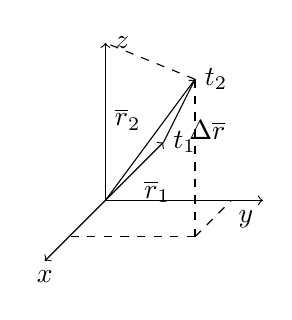
\begin{tikzpicture}[scale=0.4]
			\draw[->] (0, 0, 0) -- (5, 0, 0) node[below left] {$y$};
			\draw[->] (0, 0, 0) -- (0, 5, 0) node[right] {$z$};
			\draw[->] (0, 0, 0) -- (0, 0, 5) node[below] {$x$};

			\draw[->] (0, 0, 0) -- node[below right] {$\overline{r}_1$} (3,
			3, 3) node[right] {$t_1$};
			\draw[->] (0, 0, 0) -- node[above left] {$\overline{r}_2$} (4,
			5, 3) node[right] {$t_2$};
			\draw (3, 3, 3) -- node[below right] {$\Delta \overline{r}$} (4, 5, 3);

			\draw[dashed] (4, 5, 3) -- (0, 5, 0);
			\draw[dashed] (4, 5, 3) -- (4, 0, 3);
			\draw[dashed] (4, 0, 3) -- (4, 0, 0);
			\draw[dashed] (4, 0, 3) -- (0, 0, 3);
		\end{tikzpicture}
	\end{center}
	\caption{}%
	\label{fig:radius-vector}
\end{figure}

Любой вектор может быть задан проекциями на оси системы координат:
\begin{align*}
	\vec{r}        & = \vec{e_x}x + \vec{e_y}y + \vec{e_z}z \\
	\vec{r}        & = \vec{r}(t)                           \\
	\Delta t       & = t_2 - t_1                            \\
	\Delta \vec{r} & = \vec{r_2} - \vec{r_1}                \\
	\Delta x       & = x_2 - x_1                            \\
	\Delta y       & = y_2 - y_1                            \\
	\Delta z       & = z_2 - z_1                            \\
\end{align*}

Можно использовать разложение вектора на составляющее.

\subsection{Приращение радиус-вектора}%

Приращение радиус-вектора материальной точки в процессе её движения: \[
	\Delta \vec{r}(t) = \vec{r_0} + \Delta \vec{r}
	,\] где \( r_0 \) --- будет определять начальное положение материальной точки,
\( \Delta \vec{r} \) --- приращение в момент движения.

В общем случае путь отличается от длинны вектора перемещения. Путь \( \Delta l
\) больше или равен длине вектора \( |\Delta \vec{r}| \), если рассматривать
меньшие траектории и короткие промежутки времени, то конечное положение точки
будет приближаться к начальному, то есть разница между путём и траекторией
будет стремиться к нулю.

Средняя скорость --- это отношение перемещения к интервалу времени движения:
\begin{equation}
	% \label{eq:average-speed}
	\vec{V_\text{ср}} = \frac{\Delta \vec{r}}{\Delta t}
\end{equation}
Средняя скорость, которая определяется движением точки, описывает движение без
деталей.

При уменьшении участка траектории и постоянном вычислении средней скорости, мы
перейдём к понятию \emph{мгновенной скорости} --- это предельное значение
средней скорости при уменьшении времени интервала \( \Delta t \to 0 \),
мгновенная скорость определяется на бесконечно малом участке траектории.
\[
	\vec{V} = \lim_{t \to 0} \frac{\Delta \vec{r}}{\Delta t} = \frac{d \vec{r}}{d
		t} = \dot{\vec{r}}
	.\]

\begin{figure}[!htbp]
	\begin{center}
		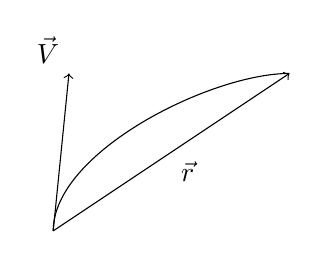
\begin{tikzpicture}
			\draw[->] (0, 0) -- node[below right] {$\vec{r}$} (3, 2);
			\draw (0, 0) .. controls (0, 1) and (2, 2) .. (3, 2);
			\draw[->] (0, 0) -- (0.2, 2) node[above left] {$\vec{V}$};
		\end{tikzpicture}
	\end{center}
\end{figure}

Если уменьшать интервал времени, то вектор \( \vec{r} \) будет приближаться к
траектории. Из определения мгновенной скорости она всегда направлена по
касательной к траектории.

Путевую скорость может показывать спидометр
автомобиля, это скалярная величина. Путевая скорость --- \( V_\text{ср} =
\frac{\Delta l}{\Delta t} - \frac{d l}{d t} \). Предельное значение предела
путевой скорости при стремлении \ldots разница между вектором \( \Delta l
\approx |\Delta \vec{r}| \), то модуль мгновенной скорости будет равен
производной пути по времени \( |\vec{V}| = \upsilon \).

Как и любой вектор скорость можно расписать как вектор или систему координат:
\( \vec{V} = V_x \vec{e}_x + V_y \vec{e}_y + V_z \vec{e}_z \). Модуль вектора
скорости (а по сути и путевой скорости) будет связан с проекциями скорости.

Зная мгновенную скорость, которая является функцией времени можно найти
изменение координат:
\begin{align*}
	\Delta x & = \int_{t_1}^{t_2} V_x(t) \\
	\Delta y & = \int_{t_1}^{t_2} V_y(t) \\
	\Delta z & = \int_{t_1}^{t_2} V_z(t) \\
\end{align*}

Равномерным называется такой вид движения, при котором за любой промежуток
времени перемещения скорость тела не изменялась. При равномерном движении
средняя и мгновенная скорости совпадают:
\begin{align*}
	x(t)       & = x_0 + \vec{V}_x t       \\
	y(t)       & = y_0 + \vec{V}_y t       \\
	z(t)       & = z_0 + \vec{V}_z t       \\
	\vec{r}(t) & = \vec{r}_0 + \vec{V}_r t \\
\end{align*}

Строго равномерным может быть только прямолинейное движение, но иногда бывает
криволинейное равномерное движение постоянство скорости по модулю. Путь же
растёт равномерно с течением времени.

Быстрота изменения скорости это и есть ускорение: \( \vec{a} = \frac{d
	\vec{V}}{d t} \). Ускорение равно нулю только в том случае, если скорость не
меняется ни по величине, ни по направлению.

Скорость можно найти, проинтегрировав ускорение:
\[
	\vec{V} = \vec{V}_0 + \int_{{t_1}}^{{t_2}} {\vec{a}(t)} \: d{t} {}
	,\] где \( \vec{a} \) --- ускорение, \( \vec{V}_0 \) --- начальная скорость.

Принципиальным вопросом в данном разделе  физики является ускорение.

\subsection{Равнопеременное движение}

\emph{Равнопеременным движением} называется равнопеременным, если за равные
интервалы происходит равное изменение скорости.

Ускорение при равнопеременном движении остаётся неизменным  (\( \vec{a} = const
\)). Примером равнопеременного движения может быть движение тел, брошенных
вблизи поверхности земли.

Характеристики движения тел вдоль осей не влияют на характеристики движения
вдоль других осей (принцип независимости движений). Следовательно, можно
рассматривать движение точки вдоль координатных осей независимо друг от друга.

% 3-я пара
\subsection{Движение по окружностям}

При движении по окружности возникают угловые кинематические характеристики:
\begin{itemize}
	\item Угловое перемещение
	\item Угловая скорость
	\item Угловое ускорение
\end{itemize}

\emph{Угловое перемещение}, если мы будем выражать его через радиус-вектор

Поворот радиус-вектора при движении по окружности будет изменяться на \( \Delta
\varphi \) за время \( \Delta t \). Чтобы указать не только величину этого
поворота, но и направление, то перемещению придают векторный характер. За
направление вектора \( \Delta \varphi \) принимается направление
поступательного перемещения правого винта.

При движении материальной точки по окружности естественно перемещение её надо
характеризовать какой--то скоростью. Тут вводится понятие угловой скорости.
Угловая скорость определяется как производная углового перемещения по времени
\[ \omega = \frac{d \varphi}{d t} .\] Направление угловой скорости будет
совпадать с вектором перемещения.

Модуль линейной скорости связан с модулем угловой скорости через радиус
окружности: \( V = \omega R \). Если линейная скорость не изменяется
по величине, то
угловая скорость также не изменяется. Для такого движения вводится понятие
равномерного движения по окружности.

При равномерном движении по окружности мы можем записать уравнение \[
	\omega = 2 \pi \nu = \frac{2 \pi}{T}
	.\] Если движения по окружности происходит с изменением угловой скорости, то
в этом случае нам надо ввести понятие углового ускорения. \emph{Угловое
	ускорение} будет определяться как \[
	\beta = \dot{\omega} = \varphi''
	.\] Аналогично случаю с линейными характеристиками \[
	\bar{\omega} = \int_{{0}}^{{t_1}} {\bar{\omega} (t)} \: d{t} {}
	.\]

При движении по окружности линейная скорость обязательно изменяется хотя бы по
направлению. По этому ускорение при криволинейном движении всегда отлично от
нуля.

Если материальная точка движется по окружности, то вектор ускорения будет
направлен по окружности.

Любой участок траектории можно представить в виде дуги окружности.

Ускорение действующее на точку, движущуюся по окружности, удобно разложить на
две составляющие. Одна из них направлена вдоль вектора скорости по касательной
к траектории (тангенциальное). Вторая в нормальном направлении к центру
окружности. Тогда у нас общее ускорение, действующее на точку, будет
определяться как сумма нормального и тангенциального ускорения.

\[
	\vec{a} = \vec{a_n} + \vec{a_\tau}
	.\]

Таким образом тангенциальная составляющая ускорения ответственна за изменения
модуля скорости. Нормальная составляющая ускорения будет определять направление
вектора.

Вектор нормального ускорения всегда перпендикулярен направлению вектора
скорости и направлен к центру ``мгновенной'' окружности. Всю траекторию
криволинейного движения можно представить как последовательность движений по
малым дугам окружностей с разными радиусами и разными положениями центров. Эти
окружности последовательно сменяют друг друга при движении точки по траектории.

Для расчёта нормального ускорения применяется формула \[
	a_n = \omega^2 R = \frac{V^2 }{R}
	.\] Для частного случая, когда происходит движение по окружности (\( R =
const \)) тангенциальное ускорение можно определить, как \[
	a_\tau = \beta R
	.\]

\subsubsection{Закон сложения скоростей в классической механике}

При рассмотрении любого вида движения его можно описывать относительно разных
систем отсчёта. По сути надо рассмотреть есть ли какая-то взаимосвязь между
кинематическими характеристиками движения в разных системах.

Пусть есть система отсчёта \( K \). Кроме этого есть система отсчёта \( K' \),
которая движется относительно системы отсчёта \( K \) с некоторой скоростью \(
U \). Положение материальной точки будет определяться радиус-вектором \( r' \).
Тогда движение материальной точки будет определяться вектором \( \bar{r} \).
Три вектора \( r_0 \), \( r \), \( r' \) связывают

В классической механике предполагается, что время в каждой системе отсчёта
течёт одинаково. В этом случае мы можем записать уравнение для скорости: \[
	\bar{V} = \bar{U} + \bar{V_\text{отн}}
	.\] Это соотношение называется законом сложения скоростей Галилея. Здесь \(
V \) --- скорость материальной точки относительно неподвижной системы отсчёта
\( K \), \( V_\text{отн} \) --- скорость материальной точки относительно
подвижной системы отсчёта \( K' \), \( U \) --- скорость движения системы \(
K' \) относительно неподвижной системы отсчёта \( K \).

\chapter{Динамика}
\section{Динамика материальной точки}%

Раздел кинематика рассматривает простейшие виды движения. При этом кинематика
не рассматривает вопросы о причинах того или иного вида движения.

Всякое тело находится в состоянии покоя или равномерно прямолинейно движется
пока воздействие на него других тел не заставит изменить это состояние.

То есть иными словами: скорость тела остаётся постоянной пока на него нет
воздействия других тел. Такое движение называется \emph{движением по инерции}.
Что бы определить не только качественную, но и количественную характеристику
движения тела (и по сути степени этого самого воздействия), то нужно ввести
понятие силы. В связи с этим сила --- мера воздействия тел друг на
друга. Если мы
говорим применяя термин мера, то значит эту величину надо как-то измерять. То
есть надо измерять меру воздействия. Существует договорённость об эталонной
мере силы, которую можно определить с помощью динамометра. Экспериментальном
же способом определяется, что сила имеет векторный характер. По скольку сила
векторная величина, то к ним можно применять правило сложения векторов.

\begin{theorem}[Первый закон Ньютона]
	Существуют такие системы отсчёта, в которых тело движется равномерно и
	прямолинейно, если на тело не  действуют другие тела или действие других тел
	скомпенсировано. Такие системы отсчёта называются инерциальными.
\end{theorem}

Важность первого закона Ньютона определяется сущностью таких систем отсчёта.
Даёт критерий выбора инерциальной системы отсчёта.

Любая система отсчёта, движущаяся равномерно относительно инерциальной системой
отсчёта тоже будет являться инерциальной.

Как будет себя вести материальная точка, если на неё будут действовать другие
тел (действие других тел не будет скомпенсировано)? Имею возможность определять
ускорение тела, а также имея возможность определять и измерять силы действующие
на тело, можно проследить взаимосвязь между силой и ускорением. Эта взаимосвязь
экспериментально установленная является содержанием второго закона Ньютона. То
есть второй закон Ньютона устанавливает связь между взаимодействием на тело и
быстротой изменения его скорости (ускорения). От сюда формулировка:

\begin{theorem}[Второй закон Ньютона]\label{thrm:second-nuton}
	В инерциальной системе отсчёта ускорение, приобретаемое материальной точкой,
	прямо пропорционально действующей на него силе.
\end{theorem}

Коэффициент пропорциональности между ускорением и действующим на него сил будет
разным для разных тел, обладающих разной инертностью.

Этот коэффициент связан с массой. Таким образом можно сказать, что масса тела
является мерой инертности тела. \[
	m = \frac{F}{a}
	.\]

По скольку ускорение и сила векторные величины, то можно записать \[
	\vec{a} = \frac{\vec{F}}{m}
	.\]

В приведённом равенстве сила. Под ней понимается равнодействующая всех сил,
действующих на тело. Происхождение этих сил может быть самой разное.

\begin{corollary}
	Второй закон ньютона не является определением силы или ускорения. Он только
	объективно связывает эти два понятия в единое целое. Каждая из входящих во
	второй закон Ньютона может быть измерена совершенно не зависимо.

	Сила, являясь количественной мерой взаимодействия тел, может вызывать как
	ускорение этих тел, так и изменение их формы. Изменение формы тел это
	деформация.
	Именно по деформации мы и определяем силу. Если взять динамометр, то там
	происходит деформация пружины.
\end{corollary}

\begin{corollary}
	Второй закон Ньютона выполняется только в инерциальных системах отсчёта, а так
	же второй закон Ньютона перестаёт работать за рамками классической механики
	(например, при скоростях, близких к скорости света (релятивистская механика);
	или же в микромире (квантовая механика)).
\end{corollary}

Второй закон Ньютона можно несколько интерпретировать:
Импульсом материальной точки называется произведение её массы на скорость \[
	\vec{p} = m \vec{\upsilon}
	.\] То есть для второго закона Ньютона можно записать \[
	m a = \frac{d P}{d t} = \vec{F}
	.\]

В аналитической форме записи ... скорость изменения импульса тела равна сумме
действующих на это тело сил.

Таким образом если известны действующие на тело силы, то мы можем определить
ускорение тела. Использую же в дополнение к этому начальные условия (начальное
положение и начальная скорость тела) можно определить зависимость координат
материальной точки от времени \[
	\vec{z} = \vec{z}(t)
	.\] А это в свою очередь называется законом движения тела. По этой причине
второй закон Ньютона называют уравнением движения. При формулировке второго
закона Ньютона всегда использовалось понятие взаимодействия. То есть любое
силовое действие носит взаимный характер.

В связи с этим можно сформулировать третий закон Ньютона:
\begin{theorem}[Третий закон Ньютона]\label{thrm:third-nuton}
	Силы взаимодействия двух материальных точек равны по величине, противоположно
	направлены и действуют вдоль одной прямой, проходящие через эти материальные
	точки.\[
		\vec{F}_{12} = - \vec{F}_{21}
		.\]
\end{theorem}

Первое тело действует на второе тело так же, как первое тело действует на
первое.

\begin{corollary}
	В классической механике предполагается, что силовое воздействие передаётся
	мгновенно даже на значительные расстояния.
\end{corollary}

При анализе движения тел приходится иметь дело с различными видами сил. Часть
сил выделена отдельно, для них определены законы. Существуют силы всемирного
тяготения. Две материальные точки притягиваются с силами, пропорциональными
произведению их масс и обратно пропорциональны квадрату расстояния между ними
\[
	F = G \frac{m_1 \cdot m_2}{R^2} \cdot \frac{\vec{r}(t)}{\vec{r}}
	.\] На второе тело действует точно такая же сила, которая будет равна
величине, но противоположна по направлению. Таким образом используя эту
формулу можно находить силу взаимного притяжения между двумя телами.

Если же по условию задачи нельзя принять за материальную точку, то в этом
случае тело надо разбить на объекты каждое из которых можно будет принять за
материальную точку, а затем суммировать все силы.

Можно использовать формулировку Всемирного тяготения для больших тел
сферической формы.

Роль величины \( R \) в данном будет выполнять расстояние между геометрическими
центрами космических тел.

\section{Упругие силы}%
% \label{sec:Упругие силы}

\emph{Упругие силы} возникают при деформации тел. В некотором интервале
деформации величина деформации пропорциональна приложенной силе (закон Гука).
Со стороны пружины действует сила реакции \[
	F_\text{упр} = k \Delta x
	,\] где \( k \) --- коэффициент жёсткости, \( \Delta x = l - l_0 \). Под
деформацией также может пониматься прогиб балки, угол закручивания стержня ну
и другие виды деформации, которые могут. При этом сила упругости всегда
противоположна направлению деформации тела. Поэтому правильнее записать \(
F_\text{упр} = - k \Delta x \).

\section{Силы трения}%
% \label{sec:Силы трения}

\emph{Силы трения} возникают при движении или при возможности движения
контактирующих друг с другом тел. В частности существует ``сухое трение'',
которое возникает при возможности движения одного тела по сухой поверхности
другого тела. Существуют случаи, когда на тело, соприкасающееся с некоторой
поверхностью, но оно остаётся в покое. Это результат того, что на тело
действует сила трения покоя, которая компенсирует другие внешние силы. Величины
силы трения покоя находится из условия относительного движения: \[
	F_\text{т.п.} + \sum_{n=1}^{i} F_i = 0
	,\] где \( F_i \) --- силы, приложенные к телу за исключением силы трения. То
есть пока тело находится в покое, сила трения в точности равна и
противоположна по направлению результирующей всех сил, действующих на тело.
Максимальное значение силы трения покоя \[
	F_\text{т.р.}^\text{max} = \mu F_N
	,\] где \( F_N \) --- нормальная составляющая реакции опоры, \( \mu \) ---
коэффициент трения поверхностей.

\begin{figure}[!htbp]
	\begin{center}
		\begin{tikzpicture}[scale=0.7, transform shape]
			\draw[->] (-1, 0) -- (5, 0) node[below right] {$\sum F_i$};
			\draw[->] (0, -1) -- (0, 3) node[left] {$F_\text{тр}$};

			\draw (0, 0) -- node[below right] {тело в покое} (2, 2) -- node[above]
			{тело скользит} (5, 2);
			\draw[dashed] (2, 0) -- (2, 2) -- (0, 2) node[left] {$\mu F_N$};
		\end{tikzpicture}
	\end{center}
	\caption{График зависимости силы трения от приложенных сил}%
	\label{fig:depends-Ftr-Fi}
\end{figure}

То есть до какого-то значения сила трения возрастает, а после начала движения
остаётся в покое (смотреть рисунок~\ref{fig:depends-Ftr-Fi}). То есть наклонный
участок графика соответствует трения покоя.

С некоторой долей приближения можно считать, что сила сухого трения не зависит
от величины скорости. Чтобы придать векторный характер записи силы трения, мы
можем ввести скорость: \[
	\vec{F_\text{т. р.}} = - \mu F_N \cdot \frac{\vec{V}}{\upsilon}
	,\] где \( \vec{V} \) скорость движения, \( \upsilon \) --- модуль скорости
движения.

При движении тел в жидких или газообразных средах возникает так называемая сила
вязкого трения. Основное отличие силы вязкого трения от сухого трения в
отсутствии трения покоя и зависимости от скорости движения. При малых скоростях
сила вязкого трения пропорциональна скорости: \[
	F_\text{тр}^b = -b V
	,\] где \( b \) --- коэффициент силы вязкого трения.

\section{Динамика твёрдого тела}%
% \label{sec:Динамика твёрдого тела}

\begin{figure}[!htbp]
	\begin{center}
		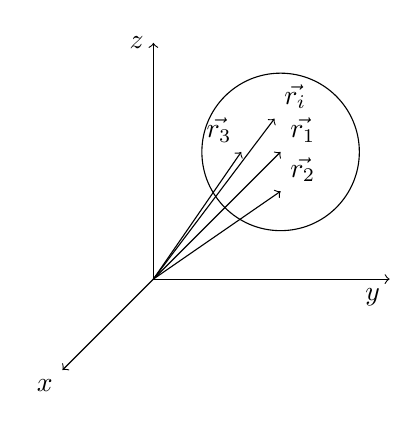
\begin{tikzpicture}[scale=1, transform shape]
			\draw[->] (0, 0, 0) -- (3, 0, 0) node[below left] {$y$};
			\draw[->] (0, 0, 0) -- (0, 0, 3) node[below left] {$x$};
			\draw[->] (0, 0, 0) -- (0, 3, 0) node[left] {$z$};

			\draw (2, 2, 1) circle (1);

			\draw[->] (0, 0, 0) -- (2, 2, 1) node[above right] {$\vec{r_1}$};
			\draw[->] (0, 0, 0) -- (2, 1.5, 1) node[above right] {$\vec{r_2}$};
			\draw[->] (0, 0, 0) -- (1.5, 2, 1) node[above left] {$\vec{r_3}$};
			\draw[->] (0, 0, 0) -- (2.5, 3, 2.5) node[above right] {$\vec{r_i}$};
		\end{tikzpicture}
	\end{center}
	\caption{}%
	\label{fig:pull-radius-vectors}
\end{figure}

Твёрдое тело можно представить как совокупность материальных точек. В этом
случае центром масс системы материальных точек называется точка, положение
которой в выбранной системе отсчёта определяет радиус-вектор. \[
	\vec{r_c} = \frac{\sum_{i=1}^{n} \Delta m_i \vec{r}}{m}
	.\] Все \( r_i \) это радиус-векторы частиц, входящих в систему (смотреть
рисунок~\ref{fig:pull-radius-vectors}). Такими частицами могут быть как
материальные точки, так и отдельные элементы на которые можно разбить твёрдое
тело.

В проекционной форме:
\begin{align*}
	x_c = \frac{\sum_{n=1}^{i} \Delta m_n x_n}{m} \\
	y_c = \frac{\sum_{n=1}^{i} \Delta m_n y_n}{m} \\
	z_c = \frac{\sum_{n=1}^{i} \Delta m_n z_n}{m} \\
\end{align*}

\emph{Импульсом} системы материальных точек называется сумма импульсов
отдельных её частей. \[
	p = \sum_{n=1}^{i} \Delta m_n V_n
	.\] Для твёрдого тела в левой части равенства оказывается произведение центра
масс на его скорость: \( p = m V_c \). Но такой результат справедлив только
для твёрдого тела.

\begin{figure}[!htbp]
	\begin{center}
		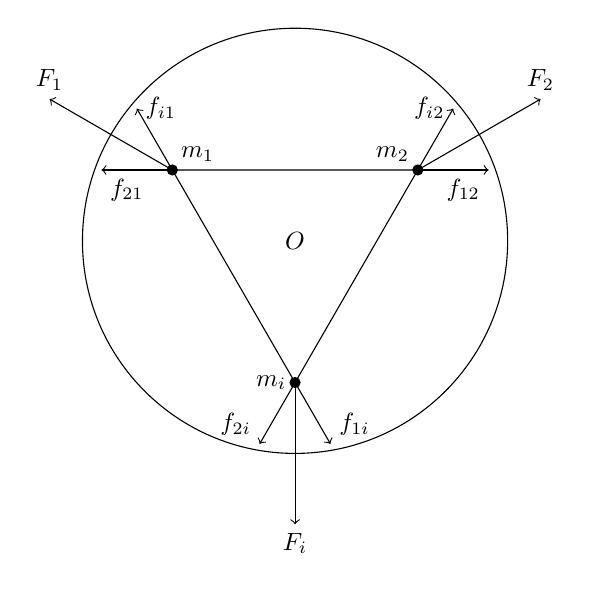
\begin{tikzpicture}[scale=0.9, transform shape]
			\draw (0, 0) circle (3);

			\coordinate (P1) at (150:2);
			\coordinate (P2) at (30: 2);
			\coordinate (Pi) at (0, -2);

			\node (O) at (0, 0) {$O$};

			% треуугольник
			\draw (P1) -- (P2) -- (Pi) -- cycle;
			\draw[fill=black] (P1) circle (2pt);
			\draw[fill=black] (P2) circle (2pt);
			\draw[fill=black] (Pi) circle (2pt);
			\node[above right] at (P1) {$m_1$};
			\node[above left] at (P2) {$m_2$};
			\node[left] at (Pi) {$m_i$};

			% внутренние силы
			\draw[->] (P1) -- +(180:1) node[below right] {$f_{21}$};
			\draw[->] (P1) -- +(120:1) node[right] {$f_{i1}$};
			\draw[->] (P2) -- +(0:1) node[below left] {$f_{12}$};
			\draw[->] (P2) -- +(60:1) node[left] {$f_{i2}$};
			\draw[->] (Pi) -- +(240:1) node[above left] {$f_{2i}$};
			\draw[->] (Pi) -- +(300:1) node[above right] {$f_{1i}$};

			% Внешние силы
			\draw[->] (P1) -- +(150:2) node [above] {$F_1$};
			\draw[->] (P2) -- +(30:2) node [above] {$F_2$};
			\draw[->] (Pi) -- +(270:2) node [below] {$F_i$};
		\end{tikzpicture}
	\end{center}
	\caption{Внешние и внутренние силы}%
	\label{fig:inner-outer-force}
\end{figure}

\begin{theorem}[движение центра масс]
	Силы \( f \) мы называем внутренними силами, а силы \( F \) внешними. Для
	рассматриваемого тела можно записать следующую систему уравнений \[
		\begin{cases}
			m_1 r_1'' = f_{12} + f_{21} + \ldots + f_{11} + F_1 \\
			m_2 r_2'' = f_{21} + \ldots + f_{2i} + F_1          \\
		\end{cases}
		.\] В левой части у нас пресутсвуют сумма всех внутренних сил, действующих
	на эту точку, а также внешняя сила \( F_i \). Так же под силой \( F_i \)
	может пониматься равнодействующая общая сила.
\end{theorem}

\emph{Центр масс} системы материальных точек (то есть твёрдого тела) движется
также, как и материальная точка массы \( m \) под действием тех же внешних сил,
которые действуют на систему.\[
	a_c = \frac{\sum_{i=1}^{n} F_i}{m}
	.\] Если нам известны начальные условия и силы, действующие на твёрдое тело,
то мы можем записать закон движения центра масс этого твёрдого тела.

Для анализа движения материальной точки достаточно таких понятий, как сила,
масса и импульс. Если же мы рассматриваем движение твёрдого тела, то кроме
самих сил важны ещё точки их приложения. Кроме этого важна не только масса
тела, но и то как она распределена по отношению к возможным осям вращения.

% рисунок 4

На тело действует сила \( F \). Соответственно от оси вращения есть какой-то
радиус-вектор \( \vec{r} \). В этом случае моментом силы \( M \) относительно
некоторой точки будет векторное произведение радиус-вектора, проведённого в
точку приложения силы, на вектор этой силы. \[
	\vec{N} = [ \vec{r} \vec{F}]
	.\] Если мы говорим о переходе от векторных величин к величине по модулю, то
у нас будет \[
	N = r \cdot F \cdot \sin{\alpha} = d F
	.\]

\emph{Момент импульса} для материальной точки относительно в точки в
пространстве \( O \) будет векторное произведение радиус-вектора, проведённого
из точки \( O \) к материальной точке, на импульс материальной точки
\begin{equation}
	\label{eq:moment-impuls}
	\vec{M} = [\vec{r} \cdot \Delta m \cdot \vec{V}]
\end{equation}
Момент импульса системы материальных точек относительно точки \( O \)
будет называться суммой моментов импульсов отдельных элементов твёрдого тела
относительно этой же точки.

Для каждого из рассмотренных векторов (момент силы, момент импульса, \dots)
можно говорить о проекциях на ту или иную координатную ось. В этом случае
говорят о моменте относительно оси (или кратко его называют осевым моментом).
При чём соответствующие величины будут уже скалярными величинами.

\subsection{Уравнение моментов}%
% \label{sub:Уравнение моментов}

\paragraph{Уравнение моментов для материальной точки}

Если мы возьмём производную правой и левой частей
системы~\ref{eq:moment-impuls}: \[
	\frac{d M}{d t} = [\vec{r}' \cdot \Delta m \cdot \vec{V}] +
	[\vec{r} \cdot \Delta m \cdot \vec{V}]
	.\] В первом слагаемом получается 0, так как происходит умножение
однонаправленных векторов. Скорость изменения момента импульса частицы равна
моменту силы, действующем на эту частицу. Все моменты в этом уравнении должны
рассчитываться относительно одной точки в пространстве, неподвижной в данной
системе отсчёта.

\paragraph{Уравнение моментов для твёрдого тела}

\begin{equation}
	\frac{d M_i}{d t} = \sum_{i=1}^{n} N_i^\text{внутр} +
	\sum_{i=1}^{n} N_i^\text{внеш}
\end{equation}

То есть для каждой частицы системы мы вправе записать своё уравнение моментов.

В правой части уравнения у нас возникают суммы внешних и внутренних моментов.
Сумма всех внутренних элементов равна нулю. Тогда в правой части выражения
остаётся только сумма всех внешних моментов \[
	\frac{d M}{d t} \sum_{i=1}^{n} N_i^\text{внеш}
	.\] Скорость изменения момента импульса системы материальных точек равна
сумме моментов внешних сил, действующих на все точки этой системы. Это
уравнение справедливо только для случая движения твёрдого тела. Опять же
следует помнить, что уравнение моментов, как и в случае с материальной
точкой, справедливо в инерциальной системе отсчёта. И векторное равенство для
моментов, записанное относительно точки \( O \) можно также спроецировать на
некоторую ось, которая содержит эту точку. В этом случае мы получаем
скалярную запись уравнения моментов.

\section{Вращение твёрдого тела относительно закреплённой оси}

Рассмотрев такое понятие, как центр масс и уравнение моментов, можно
проанализировать ситуацию, в которой тело вращается вокруг закреплённой оси.
\[
	\frac{dM}{d t} = N_\text{внеш}
	.\] Осевой момент--импульс это по сути момент импульса твёрдого тела вокруг
неподвижной оси: \[
	\frac{dM_z}{d t} = N_\text{внеш}^z
	.\] Для того чтобы посмотреть вращение тела мы обычно разбиваем тело на $n$
участков. Положение каждой из них будет определяться радиус-вектором $\vec{r}$.

\begin{figure}[!htbp]
	\begin{center}
		\begin{tikzpicture}[scale=0.55]
			\coordinate (O) at (0, 4);
			\coordinate (omega) at (0, 6.5);
			\coordinate (M) at (-2, 6);
			\coordinate (dM) at (2, 6);

			% Подшипники
			\node[above right] (0, 1) {$z$};
			\draw[pattern=north west lines] (0.1, 0) rectangle +(2, 0.25);
			\draw[pattern=north west lines] (-0.1, 0) rectangle +(-2, 0.25);
			\draw[pattern=north west lines] (0.1, 8) rectangle +(2, 0.25);
			\draw[pattern=north west lines] (-0.1, 8) rectangle +(-2, 0.25);

			\draw (0, 0) -- (0, 8.25);
			\draw[] (O) ellipse (2 and 3);
			\node[below left] at (O) {$O$};

			\draw[thick, ->] (O) -- (omega) node [left] {$\vec{\omega}$};
			\draw[->] (O) -- (M);
			\node[below left] at (M) {$M_1$};
			\draw[->] (O) -- node[below] {$\vec{r}$} (dM);
			\node[below right] at (dM) {$\Delta m_1$};

			\draw (0, 5) arc (90:135:1) node[above] {$\alpha$};
			\draw[->] (0, 6) -- node[above] {$R'$} (dM);
		\end{tikzpicture}
	\end{center}
	% \caption{}%
	% \label{fig:}
\end{figure}

При вращательном движении все точки тела будут характеризоваться одним и тем же
вектором угловой скорости. Все точки тела обладают угловой скоростью. Векторы
линейной скорости и импульсов каждой из точек будут перпендикулярны как оси
$z$, так и радиус-векторам $r_i$. Проекция момента импульса каждого элемента на
ось будет равна произведению его модуля на косинус угла.

% Момент импульса осевой\\ \pattern=north west lines( M_z = M_1 \cos \alpha \).
Проекция момента импульса каждого элемента на ось будет равна произведению его
модуля на \( \cos \alpha \): \[
	M_z = M_1 \cdot \cos \alpha
	.\]

Момент импульса мы можем расписать, как \( M_z = \vec{r} \Delta m_1 \upsilon_1
\cos \alpha \). В данном выражении мы можем поменять местами множители: \( M_z
= \Delta m_1 \upsilon_1 \vec{r} \cos \alpha \). Вместо линейной скорости мы
можем записать произведение угловой скорости на радиус: \( M_z = \Delta m_1
\omega R \vec{r} \cos \alpha \). Радиус-вектор умноженный на $\cos \alpha$ по
сути тот же радиус: \( M_z = \Delta m_1 \omega R^2 \).

Для того чтобы все эти выводы перенести на всё тело, нам надо просто
просуммировать все значения: \[
	M_z = \sum_{i=1}^{n} (\Delta m_i r_i^2) \omega
	.\] Величину в скобках мы определяем как момент инерции твёрдого тела. То
есть момент инерции твёрдого тела вокруг оси $z$ --- сумма произведения масс
каждой точки тела на квадраты их расстояния от оси $z$. Момент инерции
величина скалярная.

Если производить вращение вокруг закреплённой оси, то в предельном случае мы
должны перейти не к суммированию, а к интегралу: \[
	I_z = \sum_{i=1}^{n} (\Delta m_i R_i^2) = \int_{{1}}^{{n}} {\Delta m_i R_i^2}
	,\] где $I_z$ --- момент инерции.

Импульс тела у нас определяется \( P = m \upsilon \). Осевой момент импульса
тела у нас определяется, как \[
	M_z = I_z \cdot \omega
	,\] где $\omega$ --- угловая скорость. Можно заметить, что осевой момент
импульса определяется практически точно также, как импульс тела.

Скорость изменения импульса будет равна произведению массы тела на ускорение:
\( \frac{d P}{d t} = m \vec{a} \). Для осевого момента импульса можно проделать
то же самое: \( \frac{d M}{d t} = I_z \vec{\beta} \). То есть скорость
изменения углового момента импульса равна произведению момента инерции твёрдого
тела на его угловое ускорение. То есть момент инерции твёрдого тела при
вращательном движении играет роль, аналогичную массе при поступательном
движении. При поступательном движении мера инертности --- масса, а при
вращательном --- момент импульса. Не стоит забывать, что момент инерции зависит
не только от массы, но и от распределения массы. То есть момент инерции будет
тем больше, чем большая часть массы удалена от оси вращения.

Изменение момента импульса у нас равно моменту внешних сил. Тогда мы можем
дополнить одно из предыдущих уравнений: \( i_z \vec{\beta} = N_\text{вн (z)}\).
Это уравнение носит называние основного уравнения вращательного движения.
% предложение
Однако не стоит забывать, что в этих уравнения аналогия будет не полная.
Изменение же момента импульса величина скалярная. В выражении второго закона
ньютона масса не зависит от вектора. Момент же инерции значительно зависит от
выбора оси $z$, именно по этому его называют осевым моментом инерции.

\begin{figure}[!htbp]
	\begin{center}
		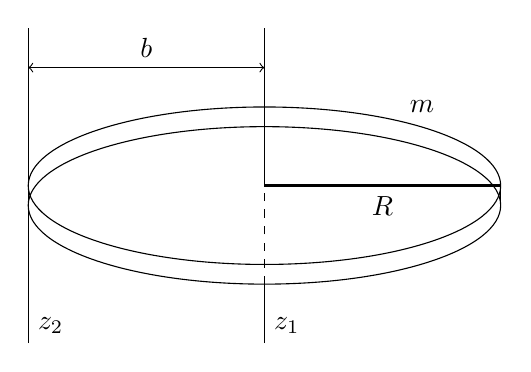
\begin{tikzpicture}[scale=1, transform shape]
			\draw(0, 0) node[above right] {$z_2$} -- (0, 4);

			\draw(3, 2) ellipse (3 and 1);
			\draw(3, 1.75) ellipse (3 and 1);
			\draw(6, 1.75) -- +(0, 0.25);

			\draw[very thick] (3, 2) -- node[below] {$R$} (6, 2);
			\draw (3, 2) -- (3, 4);

			\draw(3, 0) node[above right] {$z_1$} -- (3, 0.75);
			\draw[dashed] (3, 0.75) -- (3, 2);

			\node at (5, 3) {$m$};

			\draw[<->] (0, 3.5) -- node[above] {$b$} (3, 3.5);
		\end{tikzpicture}
	\end{center}
\end{figure}

Если у нас ось вращения проходит через центр масс диска, то момент инерции
вращения диска будет рассчитываться достаточно просто: \( I = \frac{m R^2}{2}
\). Если ось не проходит через центр масс, то на помощь приходит теорема
Гюйгенса-Штейнер.

% рисунок 3

\begin{theorem}[Теорема Гюйгенса-Штернера]\label{thrm:shteiner}
	Момент инерции тела относительно произвольной оси равен произведению моментов
	инерции тела относительно оси, параллельного данной, и проходящей через его
	центр масс и произведению массы тела на квадрат расстояния между осями.

	\begin{equation}
		I_x = I + m b^2
	\end{equation}
\end{theorem}

Для различных тел вращения просчитаны формулы расчёта момента вращения.

Для материальной точки момент инерции рассчитывается по формуле \( I
= m R^2  \).

Найдём момент инерции для цилиндра, лежащего на боку: \( I = \frac{m l^2
}{12} \).

Шар: \( I = \frac{2}{5} m R^2  \).

\section{Законы сохранения в механике}

Для того чтобы продолжить рассмотрение, нужно вспомнить
рисунок~\ref{fig:inner-outer-force}. Для каждой из материальных точек, на
которые мы разбили твёрдое тело, можно записать уравнения по второму закону
Ньютона.

\begin{theorem}[Закон сохранения импульса]\label{thrm:keep-moment-impuls}
	Тогда для одной частицы мы получаем равенство, что изменение
	импульса во времени
	будет равно сумме внешних сил: \( \frac{d P}{d} = \sum F_\text{внеш} \). Если
	сумма всех внешних сил, действующих на тела системы, то импульс системы не
	меняется с течением времени, то есть сохраняется.

	\begin{corollary}
		Закон сохранения импульса имеет те же самые границы применимости,
		что и второй
		и третий законы Ньютона. То есть по первому закону Ньютона всё у нас должно
		происходить в инерциальных системах отсчёта. То есть закон
		сохранения импульса
		будет справедлив только в инерциальных системах отсчёта.
	\end{corollary}

	Для замкнутой системы материальной точки при вращении твёрдого тела
	выполняется
	уравнение моментов. Если сумма моментов внешних сил, действующих на тела
	системы, равна нулю, то момент системы не меняется с течением времени, то
	момент импульса сохраняется.

	\begin{corollary}
		Момент импульса системы сохраняется в инерциальной системе отсчёта. В этой
		системе точка $O$ (точка, через которую проходит ось вращения
		тела) покоится.
		Относительно этой оси через точку определяется момент $P$ и все моменты
		действующих на тело внешних сил.
	\end{corollary}

	\begin{corollary}
		Требование к тому, чтобы сумма внешних сил была равна нулю очень жёсткое.
		Если равна нулю сумма проекций внешних сил на некоторое направление, то
		сохраняется проекция момента импульса системы только на это направление.
	\end{corollary}

\end{theorem}

\section{Работа силы}%

Если сила действует на движущиеся тело, то в это случае говорят, что она
совершает работу. При этом исключением является тот случай, когда сила
действует перпендикулярно вектору скорости. В процессе движения как величина,
так и взаимные направления векторов силы и скорости могут меняться. Если
вспомнить простейший случай прямолинейного движения под действием постойной
силы.

\begin{figure}[!htbp]
	\begin{center}
		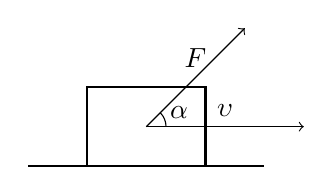
\begin{tikzpicture}[scale=0.5]
			\draw (-3,0) -- (3, 0);
			\draw[thick] (-1.5, 0) -- (-1.5, 2) -- (1.5, 2) -- (1.5, 0) -- cycle;

			\draw[->] (0, 1) -- node[above] {$\upsilon$} (4, 1);
			\draw[->] (0, 1) -- node[above] {$F$} (2.5, 3.5);

			\draw (0.5, 1) arc (0:45:0.5) node[right] {$\alpha$};
		\end{tikzpicture}
	\end{center}
\end{figure}

В таком случае не изменяется ни сама сила, ни угол между направлением движения
и вектором силы. В этом случае определяется простым соотношением. Путь мы можем
определить как радиус-вектор.

Не стоит забывать, что работа величина скалярная. Если угол $\alpha$ острый, то
работа положительная. В противном случае работа отрицательная. Если сила
перпендикулярна направлению движения ($\alpha = \frac{\pi}{2}$) даже несмотря
на наличие действующей силы и наличие перемещения, работа такой силой не
совершается ($A = 0$).

Предположим, что тело массой $m$ будет двигаться не прямолинейно, а по какой-то
произвольной траектории (смотреть рисунок~\ref{fig:move-point-by-traeck}). В
этом случае будет меняться как направление силы, так и величина вектора силы.

\begin{figure}[!htbp]
	\begin{center}
		\begin{tikzpicture}[scale=1, transform shape]
			\draw[name path=track] (0, 0) node[below] {1} .. controls (2, 5) and (5,
			2) .. (5, 5) node[above] {2};
			\path[name path=temp] (0.1, 0.1) -- (4.9, 4.9);
			\path[name intersections={of=track and temp, by=A}];

			\draw[fill=black](A) circle (1pt);
			\node[above left] at (A) {$m$};

			\draw[->] (A) -- +(60:1) node[above] {$F$};
			\draw[->] (A) -- +(14:1);
			\draw (A) -- node[below] {$\Delta l_i$} ++(14:1) -- +(0, 0.25)
			-- +(0, -0.25);
			\draw (A) -- +(0, 0.25) -- +(0, -0.25);

			\draw (A) -- ++(14:0.5) arc (14:60:0.5) node [right] {$\alpha$};
		\end{tikzpicture}
	\end{center}
	\caption{Движение точки по криволинейной траектории}%
	\label{fig:move-point-by-traeck}
\end{figure}

В этом случае для нахождения работы силы, разбиваем траекторию на малые
участки (элементарные) $\Delta l_i$. При чём выбираем мы эти участки таким
образом, что силу на них можно считать постоянной. Тогда силу на участке
$\Delta l_i$ можно рассчитать следующим образом: \( \Delta A_i = F \Delta l_i
\cos \alpha \). Так как нам надо узнать всю работу на траектории, то необходимо
сложить все работы $\Delta A_i$: \[
	A = \sum_{i=1}^{n} F \Delta l_i \cos \alpha
	.\] Если мы будем бесконечно уменьшать участки $\Delta l_i$, то мы перейдём к
интегральным суммам. Элементарная работа в таком случае рассчитывается как
произведение проекции силы на направление малого перемещения точки приложения
силы и на модуль этого перемещения. А общая работа на конечном участке
траектории будет вычисляться, как сумма элементарных работ.
\begin{equation}
	A = \int F dl
\end{equation}

Стоит обратить внимание, что работа будет всегда зависеть от выбранной систем
отсчёта. Так же часто требуется вычислить работу для тела, вращающегося вокруг
закреплённой оси (рисунок~\ref{fig:rotating-body}).

\begin{figure}[!htbp]
	\begin{center}
		\begin{tikzpicture}[scale=0.5]
			\draw[pattern=north east lines] (-0.1, -4) rectangle +(-1, -0.5);
			\draw[pattern=north east lines] (0.1, -4) rectangle +(1, -0.5);
			\draw[pattern=north east lines] (-0.1, 4) rectangle +(-1, 0.5);
			\draw[pattern=north east lines] (0.1, 4) rectangle +(1, 0.5);

			\draw (0, -4.5) -- (0, 4.5);
			\draw[->] (0, -4.5) -- (0, 4) node[below left] {$\vec{\omega}$};
			\draw (0, 0) ellipse (2 and 3);

			\draw (0, 0) circle (2pt);
			\draw[->] (0, 0) -- node[below] {$\vec{r}$} (45:2) -- +(0, 2) node[below
					right] {$F$};
			\draw (0, 0) -- (45:2) -- node[above] {$R$} ($ (0, 0)!(45:2)!(0, 4) $);

			\draw[->] (-15:3) arc(-15:-40:4) node[right] {$\Delta \varphi$};
			\node[above left] at (-1.5, 2) {$m$};
		\end{tikzpicture}
	\end{center}
	\caption{Вращающееся тело}%
	\label{fig:rotating-body}
\end{figure}

При вращении тела у нас есть угловое перемещение $\Delta \varphi$. Работу при
повороте на конечный угол опять же можно найти, суммируя элементарные работы.
Для элементарной работы мы можем записать соответствующее выражение: \[
	A = N d \varphi
	.\] Если мы переходим от элементарной работы к работе на какой-то угол, то у
нас снова всё производится через интеграл: \[
	A = \int N d \varphi
	.\] Интеграл берётся по всем углу поворота. То есть интеграл у нас будет
меняться от $\varphi_1$ до $\varphi_2$.

Быстроту совершения работы будет характеризовать мощность силы. По этому
мощность силы будет равна работе силы, совершаемой за малый интервал времени к
этому интервалу времени: \[
	W = \frac{\Delta A}{d t}
	.\] По скольку работа у нас вычисляется через силу, а перемещение, делённое на
время это скорость, соответственно, если мы говорим о мощности, то её можно
вычислить, как произведение силы на скорость и на косинус угла $alpha$: \[
	W = F \upsilon \cos \alpha
	.\] То есть мощность определяется, как произведение векторов скорости и
перемещения.

Во многих случаях физические системы, над которыми совершают работу, могут эту
работу запасать и при определённых условиях совершать эту работу над другими
телами или системами. Вот этот самый запас работы и будет называться
механической энергией. То есть по сути энергия это тот запас, который есть у
тела или системы, а работа это изменение уровня энергии. То есть механическая
энергия это физическая величина, измеряемая запасённой работой, которая
способна совершить система тела. Энергией обладают растянутая или сжатая
пружина, притягивающиеся или отталкивающиеся тела. Кроме того энергией обладают
движущиеся тела. Поэтому можно сделать вывод, что запас работы связан как с
взаимодействием тел, так и с движением тел.

В связи с этим различают два вида энергии: потенциальную и кинетическую.

\subsection{Кинетическая энергия}

Допустим некая частица движется со скоростью $\upsilon$. Что бы затормозить
частицу в течении некоторого времени должна действовать сила. Эта сила будет
совершать работу, а частица в свою очередь может совершить точно такую по
величине же работу над телами, которые тормозят эту частицу. Эта работа будет
опять же пропорциональна тем характеристикам, которые имеет частица (масса и
скорость). Значит энергия будет пропорциональна массе и скорости: \[
	E_k = \frac{m \upsilon^2}{2}
	.\] Общее значение кинетической энергии для системы будет равна для суммы
каждой частицы системы.

Кинетическая энергия, так же как и работа, зависят от выбранной системы
отсчёта. Так же как и работа, кинетическая работа это алгебраически скалярные
величины. Они также имеют свойство аддитивности, то есть соответствующая
величина для всей системы складывается из её составляющих для отдельных частиц
системы.

\begin{theorem}[о кинетической энергии тел]%
	\label{thrm:kinetic-energy}
	Изменение кинетичес\-кой энергии системы будет равно сумме сил, действующих на
	тела системы.
\end{theorem}

Снова требуется обратить внимание, что речь идёт о суммарной работе
равнодействующих к каждому телу сил.

\subsubsection{Поступательное движение}
При поступательном движении тела в любой момент времени все элементы тела $m_i$
обладают одной и той же линейной скоростью. Это та скорость, с которой движется
центр масс тела. По этому кинетическая энергия при поступательном движении
можно определить, как \[
	T = \frac{m \upsilon^2}{2}
	.\]

\subsubsection{Вращательное движение}
При вращательном движении твёрдого тела в любой момент времени у всех элементов
тела $m_i$ будут одинаковые угловые скорости. В этом случае \( T = \frac{m
	(\omega R)^2}{2} \). Если мы раскроем скобки, а затем заменим \( m R^2 \) на
момент инерции. Соответственно для вращательного движения кинетическая энергия
будет рассчитываться как \[
	T = \frac{I \omega^2}{2}
	.\]

\subsubsection{Плоское движение}

Плоское движение можно представить как совокупность одновременно
поступательного и вращательного движения. Например, можно представить это, как
вращающееся колесо.

Кинетическую энергию такого движения можно найти, если вспомнить понятие о
мгновенной скорости и вращение относительно мгновенной оси. В этом случае в
каждый момент времени движения будет представлять поворот относительно этой
мгновенной оси.

Момент инерции тела относительно мгновенной оси вращения можно определить по
теореме Штейнера: \[
	I = I_z + mR^2
	.\] Но при этом у нас ещё, кроме поворота, у нас есть ещё линейная скорость
движения тела, то есть центр масс у нас движется с линейной скоростью. Подставив
все эти значения в уравнение для потенциальной энергии, ы получим уравнение для
расчёта кинетической энергии для плоского движения твёрдого тела.
\begin{equation}
	T = \frac{I_z \omega^2}{2} + \frac{m \upsilon^2}{2}
\end{equation}

То есть при плоском движении твёрдого тела кинетическая энергия будет рана
сумме энергии поступательного движения со скоростью центра масс и энергии
вращения относительно оси, проходящей через центр масс.

\subsubsection{Консервативные и неконсервативные силы}
Силы, работа которых не зависит от формы траектории, а определяется только
начальным и конечным положением тела называются \emph{консервативными}. И из
определения естественно следует, что работа сил при замкнутой траектории будет
равна нулю. Все остальные силы относятся к \emph{неконсервативным}.

\subsection{Потенциальная энергия}

Потенциальная энергия это энергия взаимодействия тел, она зависит только от
положения тел или их координат. Поэтому понятие потенциальной энергии имеет
смысл только для консервативных сил, работа которых зависит от положения или
координаты.

Потенциальная энергия будет измеряться работой, которую тела системы могут
совершить при изменении конфигурации. Потенциальная энергия является такой
функцией координат, что работа консервативных сил равна разности значений этой
функции при изменении положения тел системы.
\[
	A = U_2 - U_1 = \Delta U_{12}
	.\]

Работа потенциальной энергии будет положительной, если энергия в состоянии 2
больше, чем энергия в состоянии 1. Иными словами говорят, что работа
осуществляется за счёт убыли потенциальной энергии.

В случае однородного поля (например поле тяготения Земли) говорят о
потенциальной энергии системы тело--Земля. В таком случае потенциальная энергия
будет определяться, как \[
	U = m g h
	.\]

Каким образом найти потенциальную энергию, если известны консервативные
действующие силы.
И второе, зная потенциальную энергию, определить силу.

Работа консервативной силы равна убыли энергии: \( A_{12} = - \Delta U_{12} \).
Поэтому для малого перемещения элементарная работа может определяться, как \(
\vec{F}_{12} dl \). В этом случае мы получаем какое-то бесконечно малое
изменение потенциальной энергии.

Для таких случаев в математике есть градиент.

\begin{equation}
	F = - \nabla U
\end{equation}

В однородном поле можно выделить геометрическое место точек, в которых
потенциальная энергия имеет одно и то же значение. Эти точки образуют
эквипотенциальные поверхности (рисунок~\ref{fig:equipotential-surface}). При
перемещении точки вдоль эквипотенциальной поверхности её работа не меняется.

По скольку при перемещении частицы вдоль эквипотенциальной поверхности работа
не совершается, то сила направлена будет по нормали к эквипотенциальной
поверхности.

В направлении нормали изменение потенциальной энергии будет производить быстрее
всего и градиент в этом случае будет показывать направление, в котором быстрее
всего растёт потенциальная энергия. То есть градиент изменения будет определять
направление силы.

\begin{figure}[!htbp]
	\begin{center}
		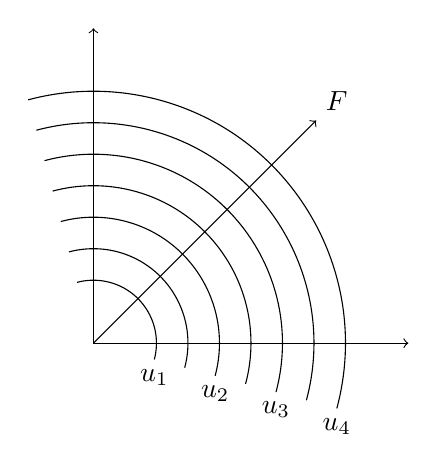
\begin{tikzpicture}[scale=0.8]
			\draw[->]  (0, 0) -- (5, 0);
			\draw[->] (0, 0) -- (0, 5);

			\foreach \i in {1, ..., 4}
			\draw (-15:\i) node[below] {$u_\i$} arc (-15:105:\i);
			\foreach \i in {1.5, 2.5, 3.5}
			\draw (-15:\i) arc (-15:105:\i);

			\draw[->] (0, 0) -- (45:5) node [above right] {$F$};
		\end{tikzpicture}
	\end{center}
	\caption{Эквипотенциальные поверхности}%
	\label{fig:equipotential-surface}
\end{figure}

В простейшем случае можно рассмотреть материальную точку, движущуюся под
действием консервативных и неконсервативных сил. По теореме о кинетической
энергии изменение кинетической энергии будет равно сумме действующих на тело
сил.

\subsubsection{Закон сохранения механической энергии}

Рассмотрим движение точки под консервативными и не консервативными силами. По
теории ~\ref{thrm:kinetic-energy} изменение равно изменению консервативных и
не консервативных сил.

Полная кинетическая энергия \( E = V + T \).

Если внешняя сила на тела системы скомпенсированы, а все внутренние силы
консервативны, то энергия системы не измена (\( E = const \)), а полная
механическая энергия сохраняется.

\section{Поле}

Для описания взаимодействия тел на расстоянии пользуются понятием \emph{силовое
	поле}. Когда рассматривают поле, то по сути считается, что тело изменяет
свойства окружающего его пространства и другие тела ``чувствуют'' это
изменение. Полю приписывается роль передатчика взаимодействия. Кроме того поле
передаёт энергию и может считаться одной из форм существования материи.

Но несмотря на все попытки создать единую теорию поля, которая бы объясняла
все явления с единой точки зрения, пока эта попытка не увенчалась успехом. Есть
отдельные частные теоретические выкладки (например, объяснение
электромагнитного поля).

Поле называется \emph{силовым}, если в каждой точке рассматриваемого
пространства определён вектор силы (причём сила эта может быть любой природы
происхождения). Силовое поле называется \emph{однородным}, если в любой его
точке на тело действует одинаковая по модулю и направлению сила. В связи с этим
любое поле в малой окрестности тела можно считать однородным.

Силовое поле будет называться \emph{центральным}, если на тело, помещённое в
поле действует сила, всегда направленная вдоль луча, соединяющего тело (ну или
точку) и центр силового поля. А величина этой силы зависит только от расстояния
от точки до центра поля. Примером такого поля как раз и служит
гравитационное поле.

Согласно закону всемирного тяготения, сила действующая на тело в гравитационном
поле определяется как \[
	F = G \frac{m M}{R^2 } \frac{\vec{r}}{r}
	.\] Данная запись означает, что действие поля распространяется мгновенно. Но в
современной физике по Эйнштейну даже световой луч должен иметь массу и быть
подвержен полю тяготения.

Силовой характеристикой любого силового поля будет являться напряжённость поля.
Для гравитационного поля эта напряжённость определяется, как \[
	g = \frac{F}{m} = G \frac{M}{R^2}
	.\] Зная напряжённость поля мы можем определить силу, действующую со стороны
поля на любое тело: \( F = m g \).

Если говорить о напряжённости гравитационного поля, то нам известно, что $g$
принимается как $9.81 \frac{\text{м}}{\text{c}^2}$.

Энергетической характеристикой поля будет являться скалярная величина, которая
называется потенциал. То есть по сути это та потенциальная энергия, которой
будет обладать в данной точке поля тело единичной массы: \[
	\varphi = \frac{U}{m}
	.\]

Для силового поля мы можем точно также рассмотреть эквипотенциальные
поверхности (смотреть рисунок~\ref{fig:equipotential-surface}). Вектор
напряжённости в каждой точке поверхности будет перпендикулярен
эквипотенциальным поверхностям, а сами эквипотенциальные поверхности
представляют собой точки равного удаления.

Силовое поле будет называться \emph{стационарным}, если его характеристики не
изменяются во времени. Для удобства силовое поле рисует с помощью силовых
линий. Касательные в каждой точке которых будут совпадать с результирующим
вектором напряжённости. При графическом изображении силового поля расстояние
между силовыми линиями поля по сути будут определять мощность поля. То есть там
где линии расположены плотнее, поле будет сильнее. Верно и обратное.

Это вызвано удобством представления при необходимости рассматривать поля,
создаваемые несколькими источниками. В этом случае результирующее напряжённость
в каждой точке находится как векторная сумма напряжённостей в этой точке
каждого из полей как если бы других полей не существовало. В этом проявляется
принцип наложения или \emph{суперпозиции} полей: \[
	g = \sum_{i=1}^{n} g_i
	.\]

То же самое можно сказать и про потенциал: \[
	\varphi = \sum_{i=1}^{n} \varphi_i
	.\]

Гравитационное поля является потенциальным. Для потенциального поля работа на
замкнутом участке пути будет равна нулю.

\chapter{Механические колебания}

Начнём рассмотрение с самого простого с математической точки зрения вида
колебаний: \emph{гармонические колебания}.

\textbf{Колебаниями} называют такие изменения физических характеристик, когда
эти характеристики периодически возвращаются в начальное состояние.

\begin{itemize}
	\item Амплитуда --- величина наибольшего отклонения от положения равновесия.
	\item Период колебаний --- время одного полного колебания.
	\item Частота колебаний --- величина, обратная периоду называется частотой.
	\item Закон изменения колеблющейся величины во времени. В случае если мы
	      говорим о гармонических колебаний, то они изменяются во времени во закону
	      синуса или косинуса;
	\item Фаза колебаний характеризует состояние колебаний в любой момент
	      времени.
\end{itemize}

\begin{figure}[!htbp]
	\begin{center}
		\begin{subfigure}{0.45\textwidth}
			\begin{center}
				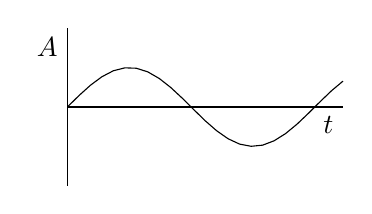
\begin{tikzpicture}[scale=0.5]
					\draw (0, 0) -- (7, 0) node[below left] {$t$};
					\draw (0, -2) -- (0, 2) node[below left] {$A$};

					\draw[domain=0:7] plot ({\x}, {sin(deg(\x))});
				\end{tikzpicture}
			\end{center}
			\subcaption{Графический вид}%
			\label{fig:graph-view}
		\end{subfigure}
		\begin{subfigure}{0.45\textwidth}
			\begin{center}
				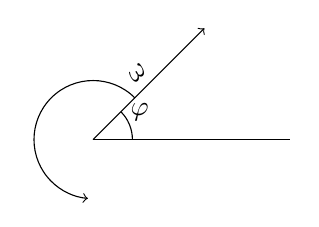
\begin{tikzpicture}[scale=0.5]
					\newcommand{\ang}{45}
					\draw(0, 0) -- +(5, 0);
					\draw[->] (0, 0) -- node[sloped, above] {$\omega$} (\ang:4);
					\draw (1, 0) arc (0:\ang:1) node[right] {$\varphi$};

					\draw[->] (\ang:1.5) arc (\ang:265:1.5);
				\end{tikzpicture}
			\end{center}
			\subcaption{Векторная вид}%
			\label{fig:vector-view}
		\end{subfigure}
		\caption{Представление колебаний}
	\end{center}
\end{figure}

Гармонические колебания могут быть представлены в одном из трёх видов:
\begin{itemize}
	\item графическом (смотреть рисунок~\ref{fig:graph-view});
	\item аналитическом: \[
		      x(t) = A \cos(\omega t + \varphi)
		      ,\] где $\varphi$ --- начальная фаза колебаний, $\omega t + \varphi$
	      --- фаза колебаний, $A$ --- амплитуда колебаний;
	\item векторном (смотреть рисунок~\ref{fig:vector-view}). В данном
	      представлении вектор вращается вокруг оси со скоростью $\omega$
	      проходящей через начало вектора. Этот вид представления удобно
	      использовать для сложения двух различных колебаний.
\end{itemize}

\section{Сложение гармонических колебаний}

Наиболее простым является случай сложение двух гармонических колебаний с
одинаковыми параметрами.

В случае аналитической записи мы имеем два колебания:
\begin{align*}
	x_1(t) & = A_1 \sin(\omega t + \varphi_1) \\
	x_2(t) & = A_2 \sin(\omega t + \varphi_2) \\
\end{align*}

По скольку оба колебания имеют одинаковые частоты, то суммарное
гармоническое колебание будет иметь туже частоту: \[
	x_1 + x_2 = A_1^2 + A_2^2 + 2 A_1 A_2 \cos (\varphi_1 - \varphi_2)
	.\]

Если мы рассматриваем колебания в графическом виде:

В векторном виде колебания складываются по правилам сложения векторов:

Величина начальной фазы результирующего колебания будет определяться как \[
	\tan \varphi_c = \frac{A_y}{A_x}
	.\] То есть в этом случае мы определили все основные параметры м=суммарного
колебания: амплитуду, частоту и начальную фазу. Но это по сути самый простой
случай, так как частоты колебаний одинаковые. Всё становится гораздо сложнее,
когда частоты разные. Практическое значение имеют те случаи, когда частоты
двух колебаний отличаются незначительно. То есть существуют два колебания,
частоты которых будут:
\begin{align*}
	\omega_1 & = \omega_0 + \Omega \\
	\omega_2 & = \omega_0 + \Omega \\
	\omega_0 & \gg \Omega          \\
\end{align*}

Для простоты возьмём, что начальная фаза одного из колебаний равна нулю:
\begin{align*}
	x_1 = A \sin(\omega_0 + \Omega) \\
	x_2 = A \sin(\omega_0 + \Omega) \\
\end{align*}

Сложив два этих выражения мы получим \[
	x_1 + x_2 = [2 A \cos (\Omega t)] \sin (\omega_0 t)
	.\]

Если амплитуды не одинаковые, то мы получим следующую картинку.

Результат суммы таких колебаний (то есть со слабо отличающимися частотами)
называется биениями. Суммарное колебание не будет являться гармоническим, хотя
в его записи и присутствует закон синуса, так как амплитуда изменятся по
какому-либо закону.

\subsection{Сложение двух взаимоперпендикулярных колебаний}

Допустим у нас есть два гармонических колебания, направления которых будет
взаимоперпендикулярно. Тогда надо взять какое-то колебание с фазой, равное нулю:
\begin{align*}
	x = a \sin(\omega t)           \\
	y = b \sin(\omega t + \varphi) \\
\end{align*}

Величина $\varphi$ будет представлять разность фаз двух колебаний.

В результате сложения \[
	\frac{x^2}{a^2 } + \frac{y^2}{b^2} - 2 \frac{x y}{a b} \cos{\omega} = \sin^2 w
\] мы получаем уравнение эллипса. При это если $\sin \varphi$ равен $0$ или
$\pi$, то в этом случае эллипс у нас вырождается в прямую. Соответственно мы
имеем:

\begin{figure}[!htbp]
	\begin{center}
		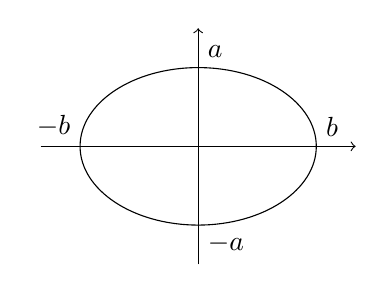
\begin{tikzpicture}[scale=0.5]
			\draw[->] (-4, 0) -- (4, 0);
			\draw[->] (0, -3) -- (0, 3);
			\draw (0, 0) ellipse (3 and 2);

			\node[above right] at (0, 2) {$a$};
			\node[below right] at (0, -2) {$-a$};
			\node[above right] at (3, 0) {$b$};
			\node[above left] at (-3, 0) {$-b$};
		\end{tikzpicture}
	\end{center}
\end{figure}

% При разности колебаний, равной $\frac{\pi}{2}$.

Если частоты складываемых колебаний отличаются друг от друга, то форма кривой
при суммировании этих двух колебаний форма у нас получается сложной. Но для
некоторых значений частот получающиеся фигуры носят называние \emph{фигуры
	Лиссажу}.


\backmatter
\printindex

\end{document}
